%
\section{Socket transfer server}

Another more general approach is to use socket communication [6] protocol. Many applications – from the networks to the mobile phones [7] use sockets. Designing software requirement is communicate with the clients and provide database information. Also keep multiple connections at the time and keep it simple.  Socket transfer server also like MySQLLIbrary was designed by using C\# programming language. It is reasonable to use one programming language during all project, therefore connection to other part be easier. \\ In general sockets very usable to use: 

\begin{itemize}
	\item Created socket transfer server and specified protocol can be used and understand by any programming language.
	\item Easy update and maintain new requirements only updates protocol specification, does not need to change server.
\end{itemize}

\subsection{Socket protocol specification}

To start design and implement our software we need to define protocol. Throw the protocol we communicate and change information. General protocol description showed in the table 7.1. Start command defines protocol type and always communication string start with 0xFE. Command type range allocated from 0x11 to 0x90, where is one byte describing command. The last one is value where is a content of data.

\begin{table}[h]
	\centering
    \begin{tabular}{ | p{4cm} | p{5cm} | p{4cm} | }
    \hline
    \textbf{Start Command} [0xFE] & \textbf{Command type} [0x11 - 0x90] & \textbf{Value}  \\ \hline
    1 byte & 1 byte & 4 or 24 bytes  \\ \hline
    \end{tabular}
	\caption{General protocol specification}
	\label{tab:protocolSpec}
\end{table}

\textbf{Example 7.1}: Subtask 4 wants to get a bin number for particular tag. So they sending string like this: 
"\textbf{0xFE 0x12} 0x30 0x30 0x30 0x30 0x31 0x32 0x33 0x34 0x31 0x32 0x33 0x34 0x41 0x41 0x31 0x32 0x33 0x34 0x35 0x36 0x41 0x34 0x35 0x36", where at the beginning defined protocol type and command type, rest of the hexadecimal values are tag id. If there are no errors in the string transfer server converts tag id to ASCII characters and sends constructed query to database. Response from database will be ASCII character which will be converted to hexadecimal and constructed packet send back to the client: "\textbf{0xFE 0x12} 0x00 0x00 0x00 0x00".

\begin{table}[h]
	\centering
    \begin{tabular}{ | p{1cm} | p{3cm} | p{3cm} | p{5cm} |}
    \hline
	& \textbf{Protocol type} & \textbf{Command type} & \textbf{Value}  \\ \hline
	Value & 0xFE & 0x12 & 000012341234AA123456A456 \\ \hline
	Bytes & 1 & 1 & 24  \\ \hline
    \end{tabular}
	\caption{Command packet (from client to server)}
	\label{tab:FromClient}
\end{table}

\begin{table}[h]
	\centering
    \begin{tabular}{ | p{1cm} | p{3cm} | p{3cm} | p{5cm} |}
    \hline
	& \textbf{Protocol type} & \textbf{Command type} & \textbf{Value}  \\ \hline
	Value & 0xFE & 0x12 & 0 \\ \hline
	Bytes & 1 & 1 & 4  \\ \hline
    \end{tabular}
	\caption{Command packet (from server to client)}
	\label{tab:FromServer}
\end{table}

\subsection{Design and implementation}

When protocol specified we can start design and implement software. Class diagram shown in the figure 7.1. \\ Here we can see four part:

\begin{enumerate}
	\item Starts server and stops main thread forever.
	\item Started server waiting for incomming packets. Incomming socket packet rises event.
	\item Transfered protocol opened and checked for incoming command. If command is not recognized then execution stoped and waiting for another incomming packet.
	\item Socket packet is class where defined buffer size, incoming client information.
\end{enumerate}

\begin{figure}[h]
	\centering
		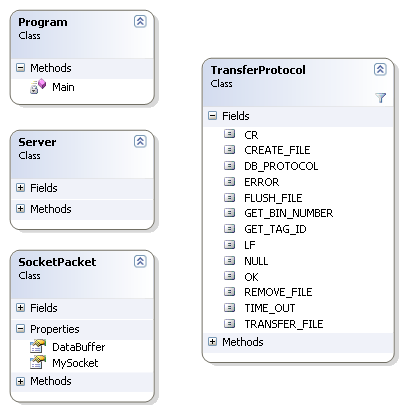
\includegraphics[scale=0.7]{socketClassDiagram}
	\caption{Class diagram of the socket transfer server}
	\label{fig:planning}
\end{figure}


\subsection{Future work}

In the future socket transfer server can be extended to have files transferring features and some security. File transferring protocol already defined however do not implemented. It could be used save elder picture. Security could be used to make safe transfer. However both of above mentioned features are not important. Picture is just additional feature and does not make sense to project. Security only necessary if transferring server will be placed out of the domain. In other case local LAN is already have security.